% **** Szablon pracy magisterskiej, licencjackiej lub inżynierskiej ****

\documentclass[polish,12pt,twoside,a4paper]{report}

% *************** Definicje stylu dokumentu ***************

% *********************************************************************************
% W pliku tym zdefiniowany jest wygląd dokumentu.
% Zmiany tutaj nie są konieczne o ile nie zamierzasz zmieniać wyglądu dokumentu.
% *********************************************************************************

% *************** Załadowanie pakietów ***************
\usepackage[a4paper,twoside,left=2.0cm,right=1.5cm,top=1.5cm,bottom=1.5cm]{geometry}
\usepackage[T1]{fontenc}
%\usepackage[cp1250]{inputenc}
\usepackage[utf8]{inputenc}
\usepackage[polish]{babel}
\usepackage{amsmath}
\usepackage{amsfonts}
\usepackage{graphicx}
\usepackage{graphics}
\usepackage{times}
\usepackage{indentfirst}%wciecia a nowych akapitach
\usepackage[hidelinks]{hyperref}

\selectlanguage{polish}

%szerokość wcięć
\setlength{\parindent}{1.25cm}

%numeracja stron
\usepackage{fancyhdr}
\pagestyle{fancy}
\fancyhf{} % usun biezace ustawienia pagin
\fancyhead[LE,RO]{ }
\fancyhead[LO]{ }
\fancyhead[RE]{ }
\fancyfoot[LE,RO]{\small\thepage}
\fancyfoot[LO]{ }
\fancyfoot[RE]{ }
\renewcommand{\headrulewidth}{0.0pt}
\renewcommand{\footrulewidth}{0.0pt}
\addtolength{\headheight}{0.0pt} % pionowy odstep na kreske
\fancypagestyle{plain}{%
\fancyhead{} % usun p. górne na stronach pozbawionych
% numeracji (plain)
\renewcommand{\headrulewidth}{0.0pt} % pozioma kreska
}

% *************** Definicje niektórych kolorów ***************
\usepackage{color}

\definecolor{greenyellow}   {cmyk}{0.15, 0   , 0.69, 0   }
\definecolor{yellow}        {cmyk}{0   , 0   , 1   , 0   }
\definecolor{goldenrod}     {cmyk}{0   , 0.10, 0.84, 0   }
\definecolor{dandelion}     {cmyk}{0   , 0.29, 0.84, 0   }
\definecolor{apricot}       {cmyk}{0   , 0.32, 0.52, 0   }
\definecolor{peach}         {cmyk}{0   , 0.50, 0.70, 0   }
\definecolor{melon}         {cmyk}{0   , 0.46, 0.50, 0   }
\definecolor{yelloworange}  {cmyk}{0   , 0.42, 1   , 0   }
\definecolor{orange}        {cmyk}{0   , 0.61, 0.87, 0   }
\definecolor{burntorange}   {cmyk}{0   , 0.51, 1   , 0   }
\definecolor{bittersweet}   {cmyk}{0   , 0.75, 1   , 0.24}
\definecolor{redorange}     {cmyk}{0   , 0.77, 0.87, 0   }
\definecolor{mahogany}      {cmyk}{0   , 0.85, 0.87, 0.35}
\definecolor{maroon}        {cmyk}{0   , 0.87, 0.68, 0.32}
\definecolor{brickred}      {cmyk}{0   , 0.89, 0.94, 0.28}
\definecolor{red}           {cmyk}{0   , 1   , 1   , 0   }
\definecolor{orangered}     {cmyk}{0   , 1   , 0.50, 0   }
\definecolor{rubinered}     {cmyk}{0   , 1   , 0.13, 0   }
\definecolor{wildstrawberry}{cmyk}{0   , 0.96, 0.39, 0   }
\definecolor{salmon}        {cmyk}{0   , 0.53, 0.38, 0   }
\definecolor{carnationpink} {cmyk}{0   , 0.63, 0   , 0   }
\definecolor{magenta}       {cmyk}{0   , 1   , 0   , 0   }
\definecolor{violetred}     {cmyk}{0   , 0.81, 0   , 0   }
\definecolor{rhodamine}     {cmyk}{0   , 0.82, 0   , 0   }
\definecolor{mulberry}      {cmyk}{0.34, 0.90, 0   , 0.02}
\definecolor{redviolet}     {cmyk}{0.07, 0.90, 0   , 0.34}
\definecolor{fuchsia}       {cmyk}{0.47, 0.91, 0   , 0.08}
\definecolor{lavender}      {cmyk}{0   , 0.48, 0   , 0   }
\definecolor{thistle}       {cmyk}{0.12, 0.59, 0   , 0   }
\definecolor{orchid}        {cmyk}{0.32, 0.64, 0   , 0   }
\definecolor{darkorchid}    {cmyk}{0.40, 0.80, 0.20, 0   }
\definecolor{purple}        {cmyk}{0.45, 0.86, 0   , 0   }
\definecolor{plum}          {cmyk}{0.50, 1   , 0   , 0   }
\definecolor{violet}        {cmyk}{0.79, 0.88, 0   , 0   }
\definecolor{royalpurple}   {cmyk}{0.75, 0.90, 0   , 0   }
\definecolor{blueviolet}    {cmyk}{0.86, 0.91, 0   , 0.04}
\definecolor{periwinkle}    {cmyk}{0.57, 0.55, 0   , 0   }
\definecolor{cadetblue}     {cmyk}{0.62, 0.57, 0.23, 0   }
\definecolor{cornflowerblue}{cmyk}{0.65, 0.13, 0   , 0   }
\definecolor{midnightblue}  {cmyk}{0.98, 0.13, 0   , 0.43}
\definecolor{navyblue}      {cmyk}{0.94, 0.54, 0   , 0   }
\definecolor{royalblue}     {cmyk}{1   , 0.50, 0   , 0   }
\definecolor{blue}          {cmyk}{1   , 1   , 0   , 0   }
\definecolor{cerulean}      {cmyk}{0.94, 0.11, 0   , 0   }
\definecolor{cyan}          {cmyk}{1   , 0   , 0   , 0   }
\definecolor{processblue}   {cmyk}{0.96, 0   , 0   , 0   }
\definecolor{skyblue}       {cmyk}{0.62, 0   , 0.12, 0   }
\definecolor{turquoise}     {cmyk}{0.85, 0   , 0.20, 0   }
\definecolor{tealblue}      {cmyk}{0.86, 0   , 0.34, 0.02}
\definecolor{aquamarine}    {cmyk}{0.82, 0   , 0.30, 0   }
\definecolor{bluegreen}     {cmyk}{0.85, 0   , 0.33, 0   }
\definecolor{emerald}       {cmyk}{1   , 0   , 0.50, 0   }
\definecolor{junglegreen}   {cmyk}{0.99, 0   , 0.52, 0   }
\definecolor{seagreen}      {cmyk}{0.69, 0   , 0.50, 0   }
\definecolor{green}         {cmyk}{1   , 0   , 1   , 0   }
\definecolor{forestgreen}   {cmyk}{0.91, 0   , 0.88, 0.12}
\definecolor{pinegreen}     {cmyk}{0.92, 0   , 0.59, 0.25}
\definecolor{limegreen}     {cmyk}{0.50, 0   , 1   , 0   }
\definecolor{yellowgreen}   {cmyk}{0.44, 0   , 0.74, 0   }
\definecolor{springgreen}   {cmyk}{0.26, 0   , 0.76, 0   }
\definecolor{olivegreen}    {cmyk}{0.64, 0   , 0.95, 0.40}
\definecolor{rawsienna}     {cmyk}{0   , 0.72, 1   , 0.45}
\definecolor{sepia}         {cmyk}{0   , 0.83, 1   , 0.70}
\definecolor{brown}         {cmyk}{0   , 0.81, 1   , 0.60}
\definecolor{tan}           {cmyk}{0.14, 0.42, 0.56, 0   }
\definecolor{gray}          {cmyk}{0   , 0   , 0   , 0.50}
\definecolor{black}         {cmyk}{0   , 0   , 0   , 1   }
\definecolor{white}         {cmyk}{0   , 0   , 0   , 0   } 

% *************** Koniec definicji stylu dokumentu ***************


%definicja przydatnych poleceń
\newcommand{\wydzial}{KOLEGIUM INFORMATYKI STOSOWANEJ}
\newcommand{\kierunek}{Kierunek: INFORMATYKA}
\newcommand{\specjalnosc}{Specjalność: Technologie IoT - Internetu Rzeczy (IoT)}
\newcommand{\autor}{Samir Al-Azazi}
\newcommand{\album}{w66045}
\newcommand{\temat}{Serwis do zwiększania jakości zdjęć}
\newcommand{\promotor}{dr inż. John Doe}
\newcommand{\typpracy}{PRACA DYPLOMOWA INŻYNIERSKA}
\newcommand{\miasto}{Rzeszów}
\newcommand{\rok}{2024}

\begin{document}

% *************** Część główna pracy ***************
% *************** Strony tytułowe ***************

% ************************************************************
% W tym miejscu znajduje sie definicja wyglądu pierwszych stron:
% strony tytułowej, strony z oświadczeniem o treści pracy
% i strony ze spisem treści
% ************************************************************
% *************** Strona tytułowa ***************
%umieszczenie logo i nazwy uczelni
\noindent
\parbox{65mm}{
\includegraphics[width=13.0cm, height=3.0cm]{logoWSIiZ}}

\vspace{10mm}
\begin{center}
{\Large{}\textbf{\wydzial}}
\end{center}
\vspace{10mm}
\noindent
\hspace{30mm}{\Large{}\textbf{\kierunek}}\\

\noindent
\hspace{30mm}{\Large{}\textbf{\specjalnosc}}
\vspace{30mm}
\begin{center}
	{\large{}\autor}\\
	{\large{}\album}\\
	\vspace{15pt}
	{\huge{}\textbf{\textit{\temat}}}\\
	\vspace{20pt}
	{\normalsize{}Promotor: \promotor}\\
	\vspace{100pt}
	{\LARGE{}\textbf{\typpracy}}\\
	\vspace{190pt}
	{\large{}\textbf{\miasto {} \rok}}
\end{center}

% pusta zawartość stopki - brak numeru strony
\thispagestyle{empty}

% *************** Strona z oświadczeniem o treści pracy ***************
\newpage
\text{}

\thispagestyle{empty}
\newpage


% *************** Spis treści ***************
\tableofcontents
% pusta zawartość stopki - brak numeru strony
\thispagestyle{empty}
\newpage

% *************** Koniec pliku front.tex ***************
\newpage
\chapter{Dynamiczne zwiększanie jakości zdjęć}

Rozwój technologii sztucznej inteligencji (AI) stanowi fundament dla licznych innowacyjnych rozwiązań w dziedzinie przetwarzania obrazów.
Jednym z fascynujących obszarów, gdzie potencjał sztucznej inteligencji jest szczególnie widoczny, jest proces dynamicznego zwiększania jakości zdjęć, nazywany również upscalingiem.
\newline
Upcaling\footnote{\href{https://en.wikipedia.org/wiki/Image\_scaling}{https://en.wikipedia.org/wiki/Image\_scaling}} to technika, która umożliwia zwiększenie rozdzielczości obrazów, co jest niezwykle istotne w kontekście poprawy detali i jakości wizualnej.
\newline
Celem niniejszego projektu jest zastosowanie zaawansowanych algorytmów opartych na sztucznej inteligencji do dynamicznego upscalingu zdjęć.
\newline
Zastosowanie technologii opartej na sztucznej inteligencji pozwala na osiągnięcie znacznie lepszych rezultatów względem tradycyjnych rozwiązań, takich jak interpolacja\footnote{\href{https://pl.wikipedia.org/wiki/Interpolacja\_(grafika\_komputerowa)}{https://pl.wikipedia.org/wiki/Interpolacja\_(grafika\_komputerowa)}}.
\newline
Projekt zakłada udostępnienie serwisu przy użyciu serwisu HTTP, który przyjmuje adres do zdjęcia, a następnie zwraca obraz w poprawionej jakości, oraz zadanej rozdzielczości.
\newline
Przeanalizujemy również już istniejące rozwiązania na rynku.

\chapter{Analiza rynku}

Stosując analizę wyników wyszukiwania popularnych wyszukiwarek (Google, DuckDuckGo, Bing), odnajdujemy wiele powtarzających się rozwiązań.
\newline
Powtarzające się wyniki we wszystkich wymienionych wyszukiwarkach to:
\begin{itemize}
	\item \href{https://www.upscale.media/}{upscale}
	\item \href{https://upscales.ai/}{upscales}
	\item \href{https://www.pixelcut.ai/image-upscaler}{image-upscaler}
	\item \href{https://www.iloveimg.com/upscale-image}{upscale-image}
\end{itemize}

Wszystkie powyższe rozwiązania dostarczają interfejs graficzny, który umożliwia użytkownikowi przesłanie zdjęcia, a następnie otrzymanie obrazu w wyższej jakości.
\newline
Wymagają również subskrypcji, w celu uzyskania dostępu do lepszej jakości, lub możliwości przetwarzania większej ilości zdjęć.
\begin{itemize}
	\item \href{https://www.upscale.media/pricing}{https://www.upscale.media/pricing}
\end{itemize}
\begin{center}
	{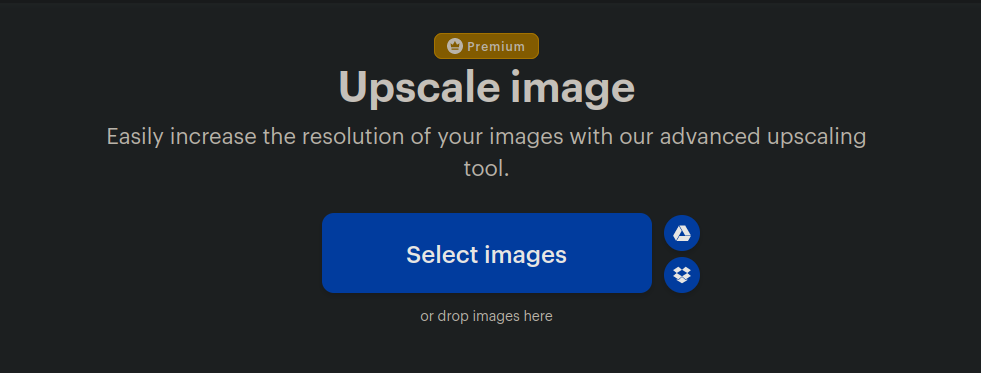
\includegraphics[width=13.0cm, height=3.0cm]{figures/upscale}}
\end{center}

\chapter{Analiza zapotrzebowania}

Bazując na formie użycia obrazów na serwisach internetowych, wymagane jest rozwiązanie, które umożliwi dynamiczne zwiększanie jakości obrazów, bez konieczności manualnej interakcji dewelopera z serwisem do zwiększenia jakości zdjęć.
\newline
Aby to osiągnąć, zostanie zaimplementowany serwis, który udostępnia interfejs HTTP, przyjmujący adres zdjęcia, które ma zostać przetworzone, oraz parametry, określające rozdzielczość wynikową.
\newline
Pozwali to na łatwą migrację istniejących serwisów, oraz bezobsługowe działanie.

\chapter{Założenia teoretyczne}

Interfejs serwisu do zwiększania jakości zdjęć, powinien akceptować adres zdjęcia, oraz rozdzielczość wynikową.
\newline
Gdy strona internetowa wyświetla obraz, który ma zostać wyświetlony w przeglądarce internetowej, do kodu HTML strony internetowej dodany jest atrybut
\newline
\begin{verbatim}
	<img src="https://ftp.pl/images/1.jpg" />
\end{verbatim}

Wskazuje on na obraz znajdujący się na serwerze \textit{ftp.pl}, pod adresem \textit{https://ftp.pl/images/1.jpg}.
\newline
Zakładając, że serwis jest dostępny pod adresem \textit{htttp://serwis.org/}, a zdjęcie, które ma zostać przetworzone znajduje się pod adresem \textit{https://ftp.pl/images/1.jpg}, to adres zwracający obraz w rozdzielczości \textit{1920x1080} to
\newline
\begin{verbatim}
	http://serwis.org/api/1920x1080/ftp.pl/images/1.jpg
\end{verbatim}

% ********** Koniec rozdziału **********
\newpage

% *************** Bibliografia ***************
\begin{thebibliography}{6}
\addcontentsline{toc}{chapter}{Bibliografia}

\bibitem{Wikipedia - Image Scalling} \href{https://en.wikipedia.org/wiki/Image\_scaling}{https://en.wikipedia.org/wiki/Image\_scaling}
\bibitem{Wikipedia} \href{https://pl.wikipedia.org/wiki/Interpolacja\_(grafika\_komputerowa)}{https://pl.wikipedia.org/wiki/Interpolacja\_(grafika\_komputerowa)}
\bibitem{HTML - Anchor} \href{https://developer.mozilla.org/en-US/docs/Web/HTML/Element/img}{https://developer.mozilla.org/en-US/docs/Web/HTML/Element/img}
\bibitem{Github - RealESRGAN} \href{https://github.com/xinntao/Real-ESRGAN/}{https://github.com/xinntao/Real-ESRGAN/}
\bibitem{W3 - Web Service} \href{https://www.w3.org/TR/2004/NOTE-ws-arch-20040211/\#relwwwrest}{https://www.w3.org/TR/2004/NOTE-ws-arch-20040211/\#relwwwrest}
\bibitem{Docs - HTTP Status} \href{https://developer.mozilla.org/en-US/docs/Web/HTTP/Status}{https://developer.mozilla.org/en-US/docs/Web/HTTP/Status}
\bibitem{Paper - RealESRGAN}\href{https://paperswithcode.com/paper/real-esrgan-training-real-world-blind-super}{Xintao Wang, Liangbin Xie, Chao Dong, Ying Shan {\it Real-ESRGAN: Training Real-World Blind Super-Resolution with Pure Synthetic Data}, 2021.1}
\end{thebibliography}
\newpage

% *************** Zakończenie ***************
% *************** Zakończenie ***************

%***************************************************************************************
% W tym miejscu znajdują się polecenia odpowiedzialne za tworzenie
% spisu ilustracji, spisu treści oraz streszczenia pracy
%***************************************************************************************

%streszczenie
\addcontentsline{toc}{chapter}{Streszczenie}
\noindent
{\footnotesize{}\textbf{Wyższa Szkoła Informatyki i Zarządzania z siedzibą w Rzeszowie\\
Kolegium Informatyki Stosowanej}
\vspace{30pt}

\begin{center}
\textbf{Streszczenie pracy dyplomowej inżynierskiej}\\
\temat
\end{center}

\vspace{30pt}
\noindent
\textbf{Autor: \autor
\\Promotor: \promotor
\\Słowa kluczowe: ai, upscalling, sztuczne sieci neuronowe, serwis http}
\vspace{40pt}
\\Treść streszczenia, czyli kilka zdań dotyczących treści pracy dyplomowej w języku polskim.
\vspace{80pt}

\noindent
\textbf{The University of Information Technology and Management in Rzeszow\\
Faculty of Applied Information Technology}
\vspace{30pt}

\begin{center}
\textbf{Thesis Summary\\}
Tytuł pracy w języku angielskim
\end{center}

\vspace{30pt}
\noindent
\textbf{Author: \autor
\\Supervisor: \promotor
\\Key words: ai, upscalling, artificial neural networks, http service}
\vspace{40pt}
\\Treść streszczenia, czyli kilka zdań dotyczących treści pracy dyplomowej w języku angielskim - tłumaczenie tekstu z języka polskiego.
}

% *************** Koniec pliku back.tex ***************


\end{document}
% *************** Koniec pliku szablon.tex ***************
